\documentclass[prc,amsmath,twocolumn,superscriptaddress]{revtex4}
%\bibliographystyle{prsty}
\usepackage{gensymb}
\usepackage{graphicx,color}
\usepackage{amssymb}
\usepackage{enumerate}
\usepackage{verbatim}
\usepackage{natbib}


\begin{document}

  \newcommand {\nc} {\newcommand}
  \nc {\Sec} [1] {Sec.~\ref{#1}}
  \nc {\IR} [1] {\textcolor{red}{#1}} 

\title{PHY905 Project 3 - Solar System}


\author{Alaina~Ross}

\date{\today}

%%%%%%%%%%%%%%%%%%%%%%%%%%%%%%%%%%%%%%%%%%%%%%%%%%%%%%%%%%%%%%%%%%%%%%%%%%%%%%%%%%%%%%%%%%%%%%%%%%%%%%%%%%%%%%%%%%%%%%%%%%%%%%%%%%%

\begin{abstract}
 \noindent {\bf Background:} A fairly accurate model of the solar system can be achieved with the use of newtonian mechanics. However, this leads to many coupled differential equations which are difficult to solve analytically.
\\ {\bf Purpose:} The goal of this work is to solve numerically the aforementioned problem. We aim to study the numerical stability of various computation methods as well as the numerical precision.
\\ {\bf Method:} We approximate the derivatives in the coupled differential equations and solve them using the Euler method and the velocity Verlet method.
\\ {\bf Results:} We find the the Euler method is unstable even in the binary Earth-Sun system, and causes non-conservation of both energy and angular momentum. In contrast, the velocity Verlet method is found to be very stable and enforces conservation of energy and angular momentum.
 \\ {\bf Conclusions:} Our results demonstrate both the importance of an effective differential equation solver, and that the sun (due to its large mass) essentially controls all of the dynamics of the other bodies in the system. 
\end{abstract}


\maketitle

%%%%%%%%%%%%%%%%%%%%%%%%%%%%%%%%%%%%%%%%%%%%%%%%%%%%%%%%%%%%%%%%%%%%%%%%%%%%%%%%%%%%%%%%%%%%%%%%%
\section{introduction}
\label{intro}
Perhaps the most fundamental question one could ask in the field of astrophysics is why the planets move the way they do. While the advanced theory of general relativity is needed to answer this question, the much simpler Newton's laws of gravitation offer a good approximation except for in large gravitational fields and at short distances, such as with the incorrect estimation of the precession of Mercury~\cite{mercury}. While these equations are much simpler, as the number of bodies in the system is increased, more and more coupled differential equations are needed, which quickly becomes analytically taxing. However, with computational methods and newtonian mechanics one can develop a fairly accurate model of the solar system. 

For simplicity, we first consider the binary Earth-Sun system where the force is given by:
\begin{equation}
F_G=\frac{GM_\odot M_E}{r^2}
\end{equation}
where G is the universal gravitational constant, $M_\odot$ is the mass of the sun $M_E$ is the mass of the earth, and $r$ is the distance between the earth and the sun. In this work we use the convenient units where the constant $GM_\odot =4\pi^2$ AU/year. Then the equations of motions for the coordinates $x_i$ are given by:
\begin{equation}
\frac{d^2\vec{x}}{dt^2} = \frac{4\pi^2}{r^2} ,\quad \frac{d^2x_i}{dt^2}=\frac{dv_i}{dt}=\frac{4\pi^2}{r^2}\frac{x_i}{r}.
\end{equation}

For a general system of N planets the total force on a given planet, $p$, is:
\begin{equation}
F_p=4\pi^2M_p\sum_{i=1}^N \frac{M_i}{M_\odot}\frac{1}{r_i^2},
\end{equation}
where $r_i$ is the distance between planets $p$ and $i$. Then, the equations of motion are given by:
\begin{equation}
\frac{d^2x_i}{dt^2}=\frac{dv_i}{dt}=4\pi^2\sum_{i=1}^N \frac{M_i}{M_\odot}\frac{x_i}{r_i^3}.
\end{equation}

%As the range of masses of the planets in the solar system is far larger than the range of distances, the sun and the largest planets should have the greatest effects on the orbits of the others bodies. 

While the gravitational potential binds the system, there is a point at which the kinetic energy of the body is large enough to escape the gravitational potential. This is known as the escape velocity, and it is given by:
\begin{equation}
\frac{1}{2}mv^2\geq \frac{GMm}{r^2} \rightarrow v_{e}=\sqrt{\frac{GM}{r}}.
\end{equation}
Then, in order to keep our system realistic and bounded, it is important that realistic initial conditions are used for each planet. To accomplish this we use the HORIZON system from the Jet Propulsion Lab at NASA~\cite{horizon}.

In this work, we implement the Euler method and the velocity Verlet method to solve the above coupled differential equations for varying number of planets. In addition, the accuracy and stability of the algorithms are investigated along with the performance. In Section \ref{methods}, the implementation of the algorithma are described. In Section ~\ref{results} the performance and accuracy of the code are analyzed. Finally, in Section \ref{conc} we give a summary and our conclusions.


\section{methods}
\label{methods}

The first method employed to solve the differential equations is the Euler method. For a given discretized function, $x(t_i)=x_i$, the Euler method involves first taylor expanding as:
\begin{equation}
x_{i+1}= x(t_i)+h\left[x (t_i)+ ... + x^{(p)}(t_i)\frac{h^{p-1}}{p!}\right] + O(h^{p+1})
\end{equation}
where h is the step size. Truncating the term in square brackets to the first term gives:
\begin{gather}
x_{i+1}= x(t_i)+hx'_i+O(h^2).
\end{gather}
This can then be used to solve for the position, and the velocity is given by Equation 4. This method has an error of $h^2$ for each step, or $Nh^2$ total. While it is easy to implement, there are possibilities of round off error which can lead the algorithm to be unstable.

The second method used to solve the differential equations is the velocity Verlet method, where the coupled differential equations are written as:
\begin{equation}
\frac{dx}{dt}=v(x,t), \quad \frac{dv}{dt}=a(x,t).
\end{equation}
The position and velocity can then be taylor expanded as:
\begin{gather}
x_{i+1}=x_i+hv_i+\frac{h^2}{2}a_i+O(h^3) \\
v_{i+1}=v_i+ha_i+\frac{h^2}{2}a'_i+O(h^3).
\end{gather}
Where the derivative of the acceleration $a'_i$ is given by:
\begin{equation}
ha'_i\approx a_{i+1}-a_i,
\end{equation}
which gives the final velocity equation as:
\begin{equation}
v_{i+1}=v_i+\frac{h}{2}\left(a_{i+1}+a_i \right) +O(h^3).
\end{equation}
While this is a more complicated method than the Euler, it is more stable and has a smaller error.

\begin{figure}[b]
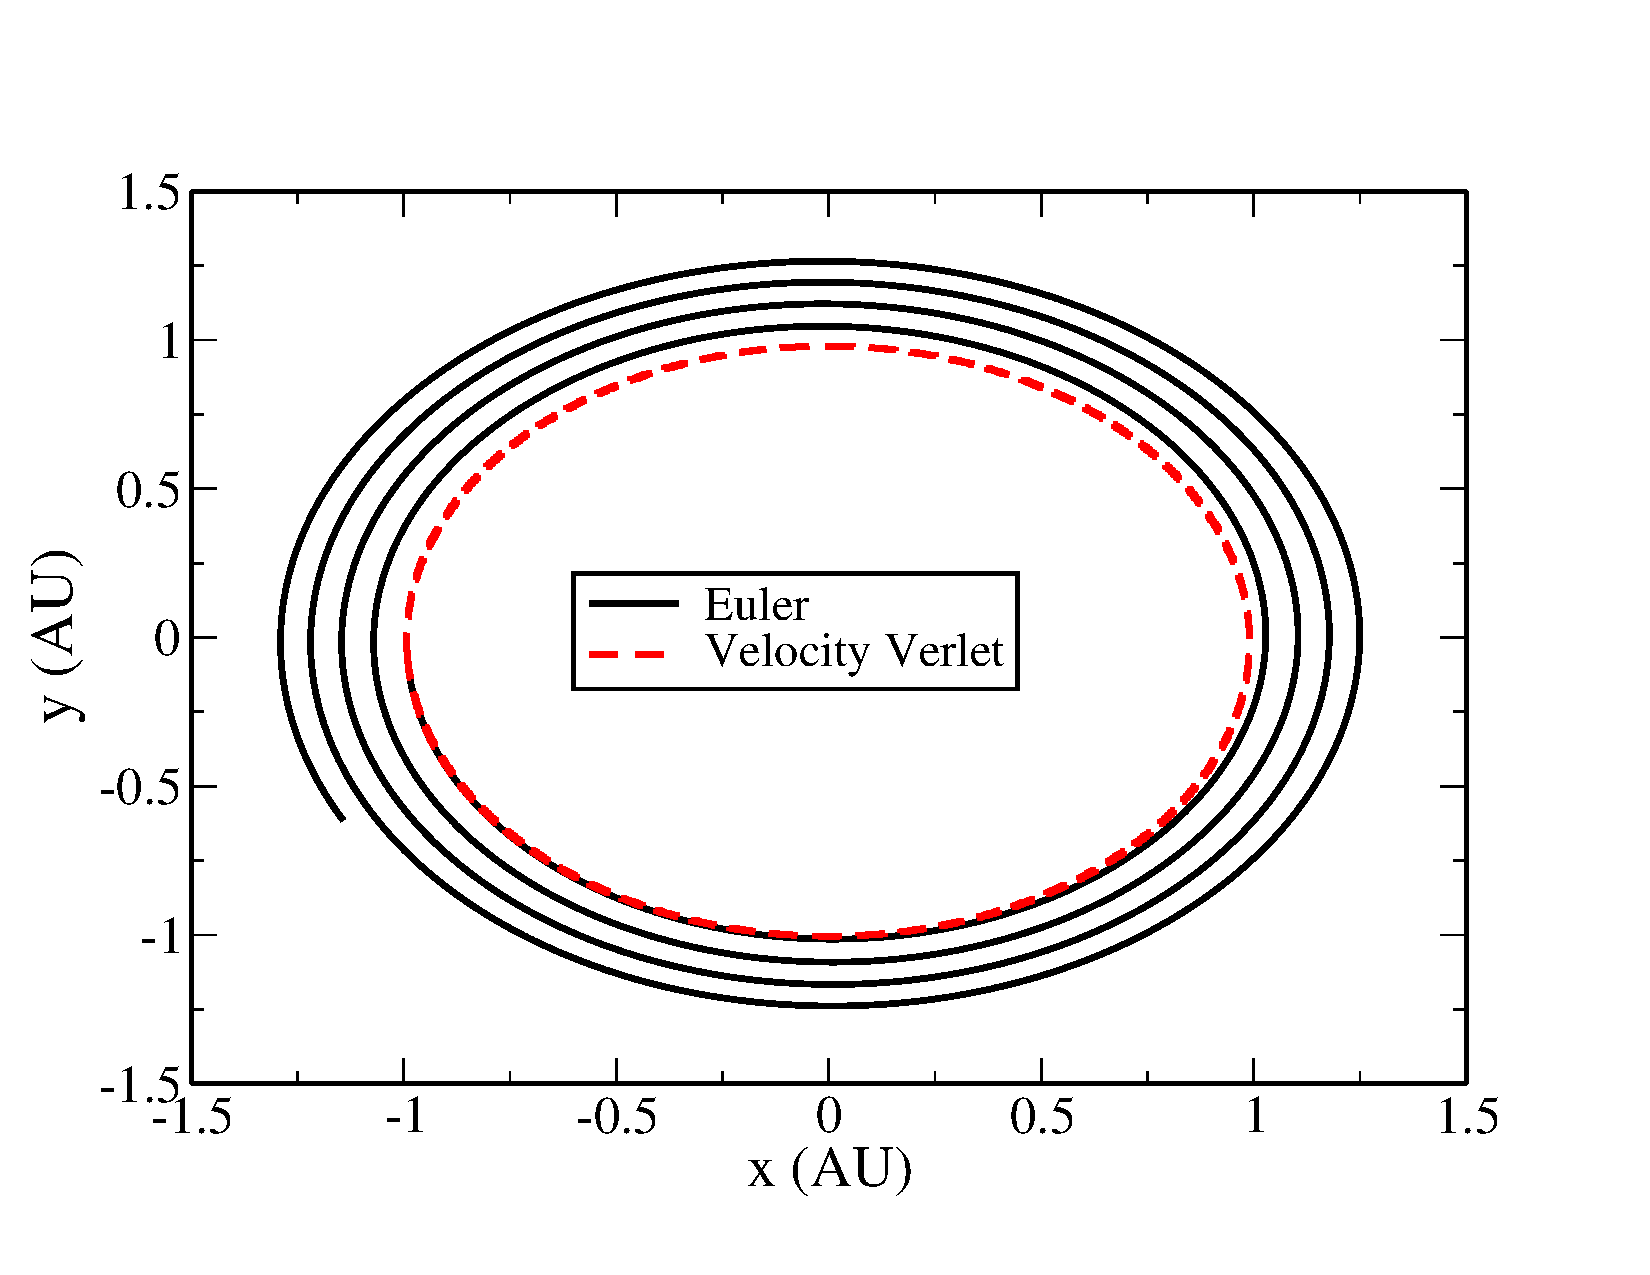
\includegraphics[scale=0.33]{binary.pdf}
\caption{Comparison of Euler and Velocity Verlet algorithms for the binary Earth-Sun system with h = 0.001 and t$_f$ = 5 years.}
\label{binary}
\end{figure}

\section{results}
\label{results}

We first use the simple binary Earth-Sun system and keep the sun fixed to compare the two methods. In Figure~\ref{binary} the motion of the Earth in the xy plane is shown for the Euler method in the black solid curve and for the velocity Verlet method in the red dashed line. The step size for the given calculation was 0.001 years, the total time was 5 years and the initial velocity of the earth is taken to be $2\pi$ AU/year to ensure a circular orbit. As is seen in the figure, the Euler method shows the Earth spiraling away from the sun, rather than in a bounded orbit as the Verlet shows. 
\begin{table}[t]
\centering
\begin{tabular}{|c|c|c|}
\hline
Quantity&~Euler~~&Velocity Verlet\\
\hline
$\Delta$Energy (\%)&23.46&0.494\\
$\Delta$L (\%)&14.17&0.272\\
Time to solution (sec)&0.164&0.488\\
%FLOPs &&\\
\hline
\end{tabular}
\caption{Comparison of Euler and velocity Verlet methods in the binary Earth-Sun system with h = 0.001 and t$_{f}$ = 5 years.}
\label{nrg}
\end{table}
As there is no torque exerted on the Earth, we expect that both energy and angular momentum should be conserved. To view this in our algorithms, we calculate the percent difference in the energy and angular momentum (L) over the course of the calculation. The results of this calculation are shown in Table~\ref{nrg}. Here we again see that the Verlet performs as expected, causing less than a half a percent change, while the Euler method causes 15-20\% changes in the given time span.

Finally, we inspect the performance of each of the algorithms via the time to solution. These are also given in Table~\ref{nrg}. While the Verlet algorithm is almost three times slower than the Euler, both times are so small that the difference is negligible. As we have shown the Euler method to be inferior to the velocity Verlet, all further calculations are done with the latter method only.

\begin{figure}[b]
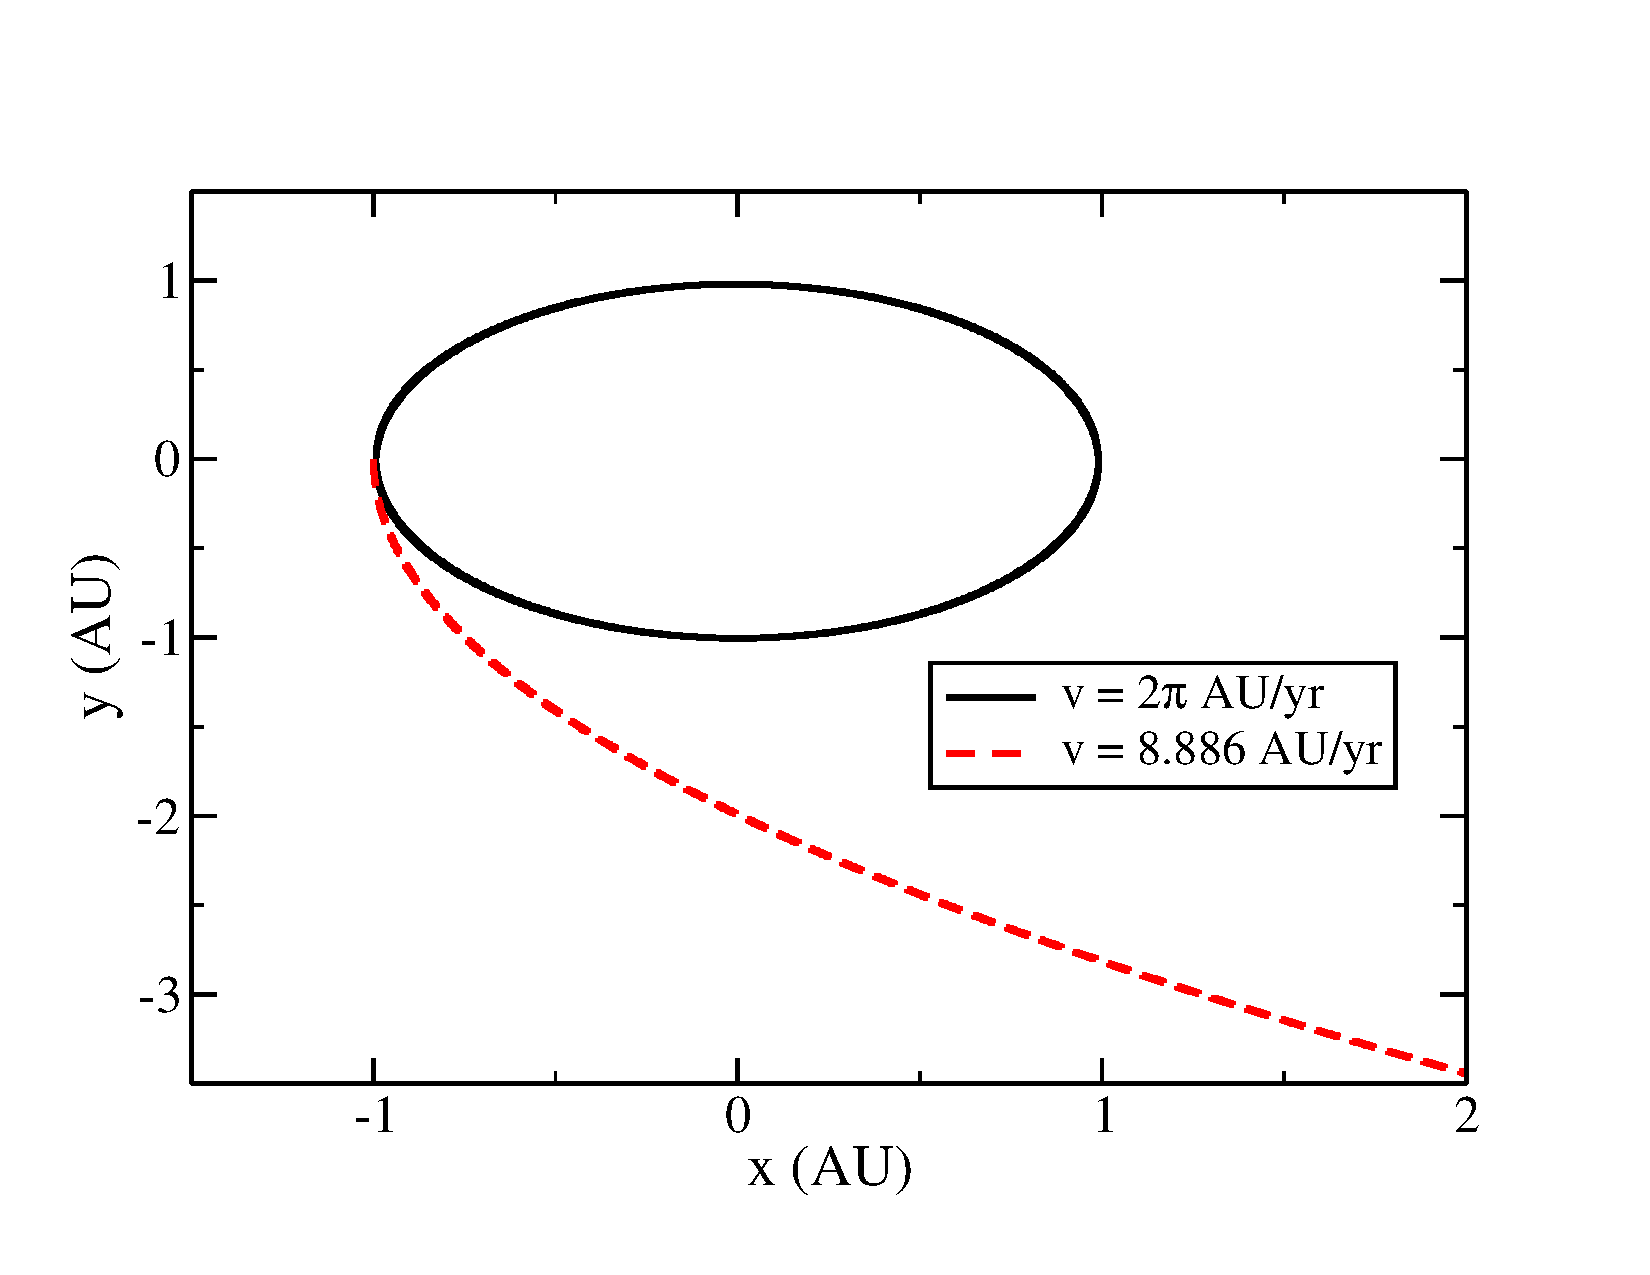
\includegraphics[scale=0.33]{escape.pdf}
\caption{Comparison of Earth's projected orbit in the binary Earth-Sun system for an initial velocity of $2\pi$ AU/year and the predicted escape velocity, 8.886 AU/year.}
\label{escape}
\end{figure}

As stated earlier, one important aspect of this calculation is ensuring that the starting velocity of any given planet is smaller than the escape velocity. For the binary system the escape velocity is calculated via Equation 5 to be 8.886 AU/year. In Figure~\ref{escape} the position of the Earth is shown for an initial velocity of $2\pi$ AU/year in the black solid curve, and with the escape velocity in the red dashed curve. Here we see that indeed with this initial velocity the Earth quickly escapes the gravitational pull of the sun and diverges.


\begin{figure}[t]
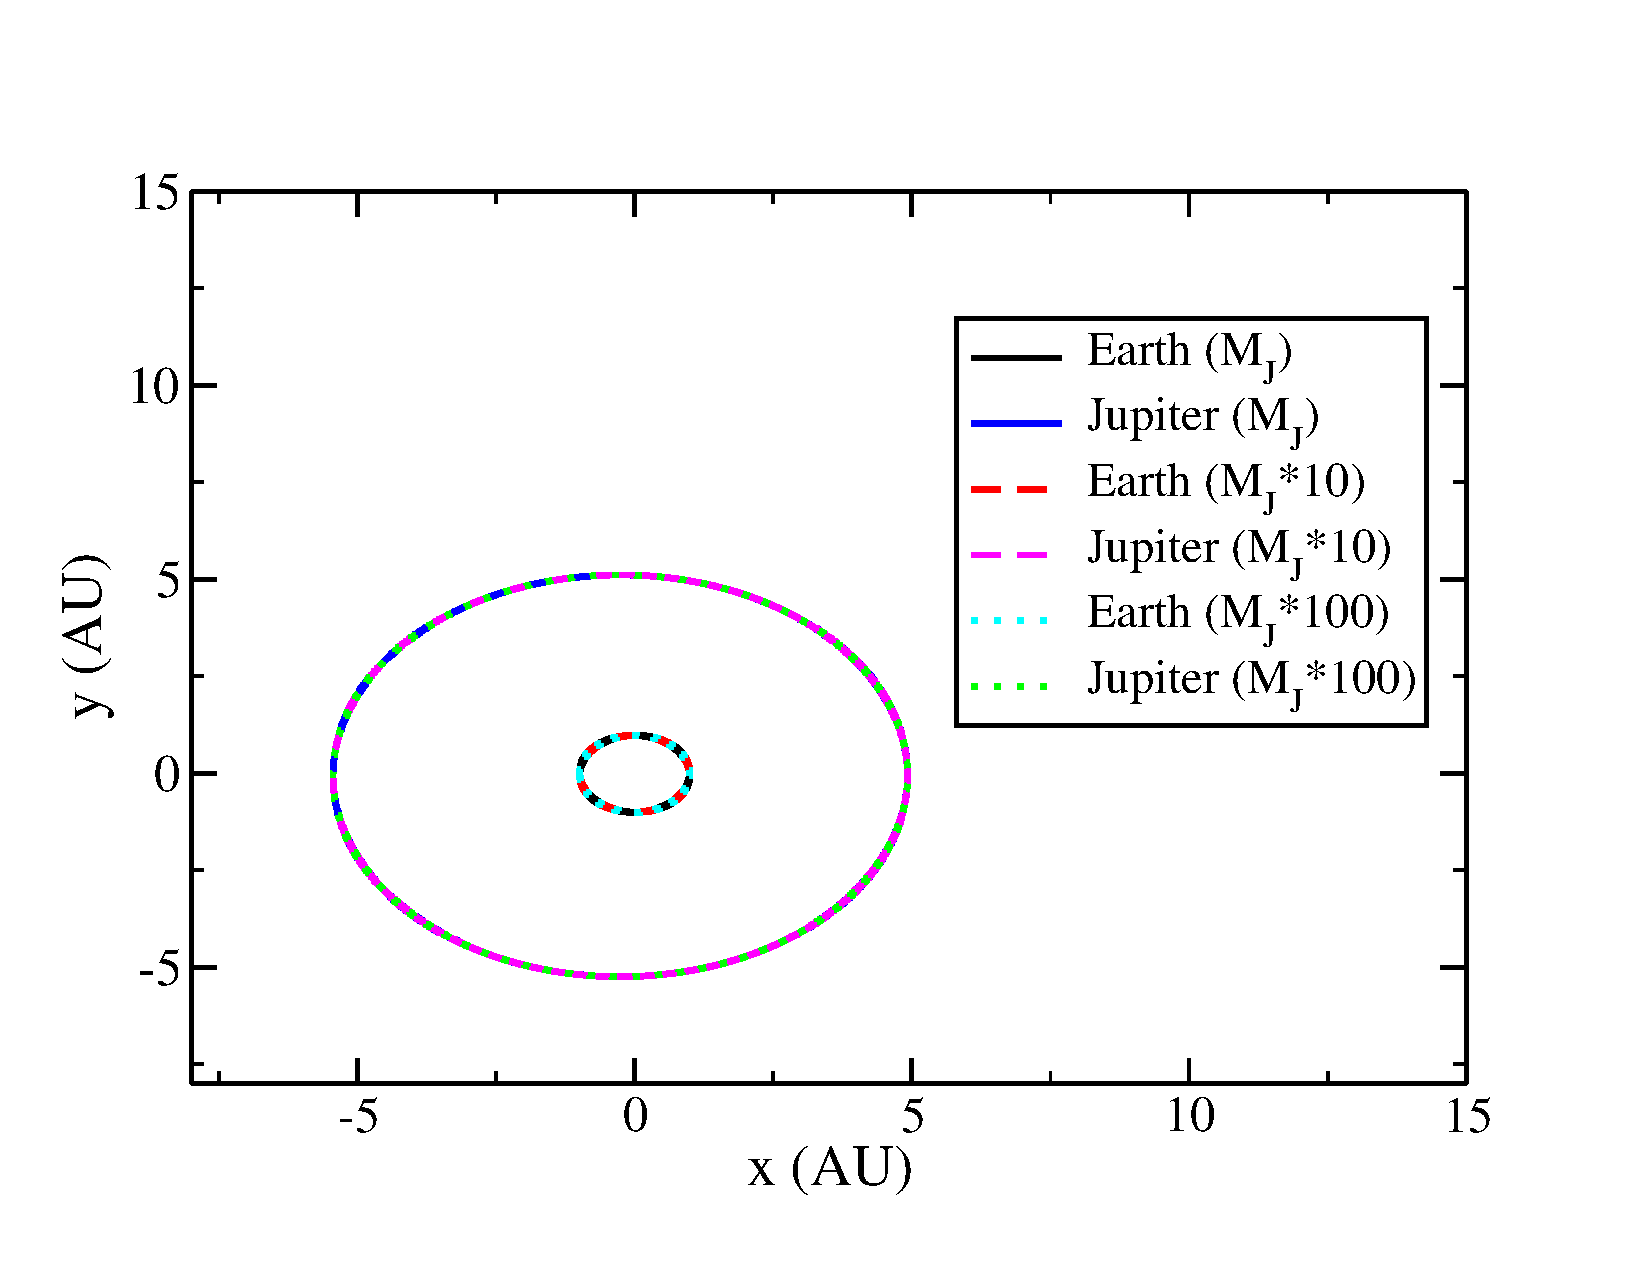
\includegraphics[scale=0.33]{three_mj.pdf}
\caption{Comparison of Earth and Jupiter's orbits in the Earth-Jupiter-Sun system for varying masses of Jupiter.}
\label{mj}
\end{figure}

After testing the algorithms with only the Earth and the sun, we add in Jupiter, the heaviest planet. As the masses of the planets in the solar system are much smaller than the mass of the sun, adding in the heaviest planet should have the largest effect on the Earths orbit. To test the sensitivity of the Earth's trajectory to the mass of Jupiter, the calculations are repeated with Jupiter having a mass 10 times larger and then 100 times larger than reality. These calculation are seen in Figure~\ref{mj}, where the black (blue) solid line is the trajectory of Earth (Jupiter) with the natural mass of Jupiter, the red (magenta) dashed line is the trajectory of Earth (Jupiter) with Jupiter's mass multiplied by ten, and the cyan (green) dotted line is the trajectory of Earth (Jupiter) with Jupiter's mass multiplied by 100, each of which is identical. This shows that the massive sun has a much greater effect on the Earth's orbit than the other planets do.

Up until now, all calculations have been performed with the sun held fixed, however, that is not the case in reality. We now allow the sun to move due to the forces exerted on it by the planets, and plot the distance from the solar system's barycenter in Figure~\ref{sun}. While the trajectory is rather elliptical, the magnitude of the orbit is much smaller than we saw previously for the Earth and Jupiter, which is to be expected.

\begin{figure}[t]
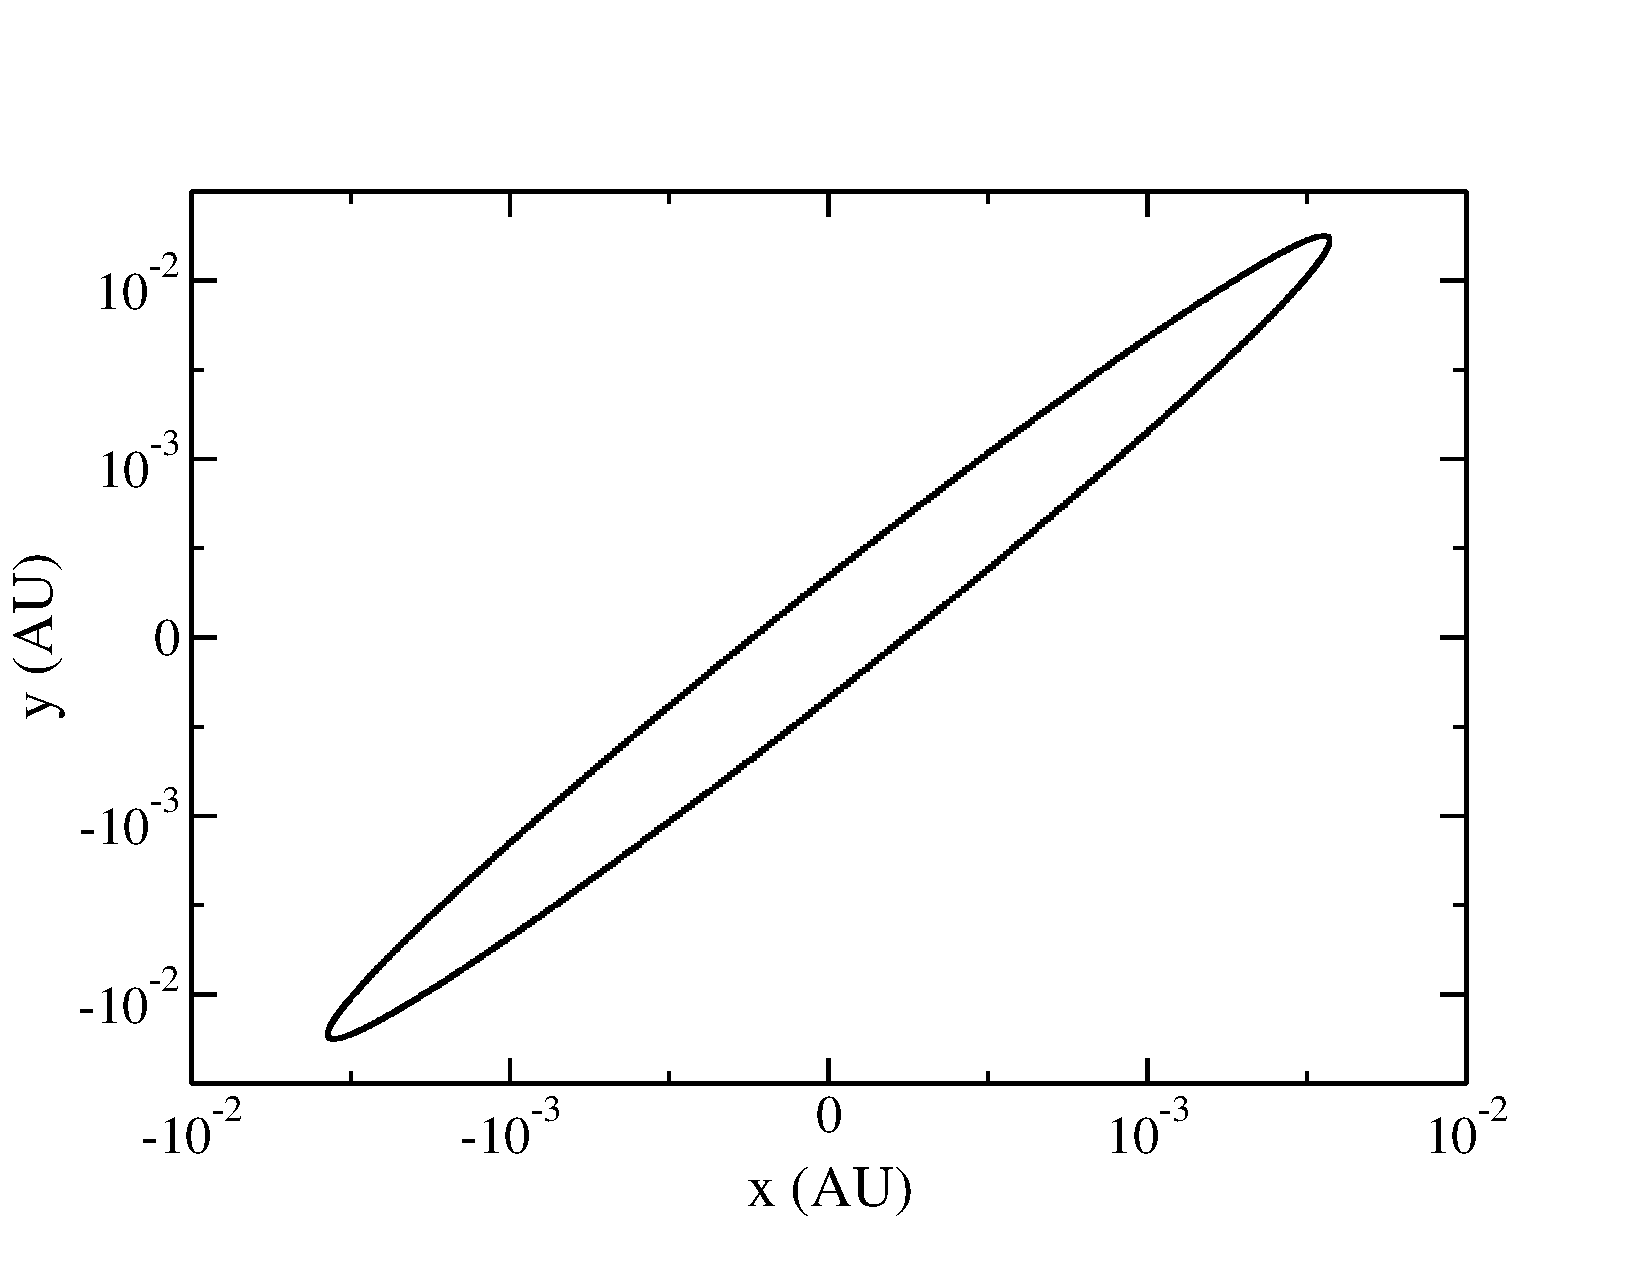
\includegraphics[scale=0.33]{sun.pdf}
\caption{Path of sun around the solar system's center of mass with all planets included.}
\label{sun}
\end{figure}

Allowing the sun to move and now including all planets in the solar system, we calculate the trajectories for each planet and show them in Figure~\ref{all}. The orange dots show the position of the sun (which appears as one dot as the trajectory is too small to be resolved), the black line corresponds to the position of Mercury, the yellow line shows Venus, the green line Earth, the blue line Mars, the brown line Jupiter, the magenta line Saturn, the red line Uranus, the purple line Neptune, and the cyan line Pluto. The inset of the plot shows the smaller orbits with more detail. The distance between each planet and the sun is compared to the expected value in Table~\ref{comp}.

\section{conclusions}
\label{conc}

In summary, the goal of this work was to calculate %numerically the paths of the planets in the solar system using Newton's law of gravitation. Two methods to calculate the differential equations were used, namely, the Euler method and the velocity Verlet method.

\begin{figure}[h]
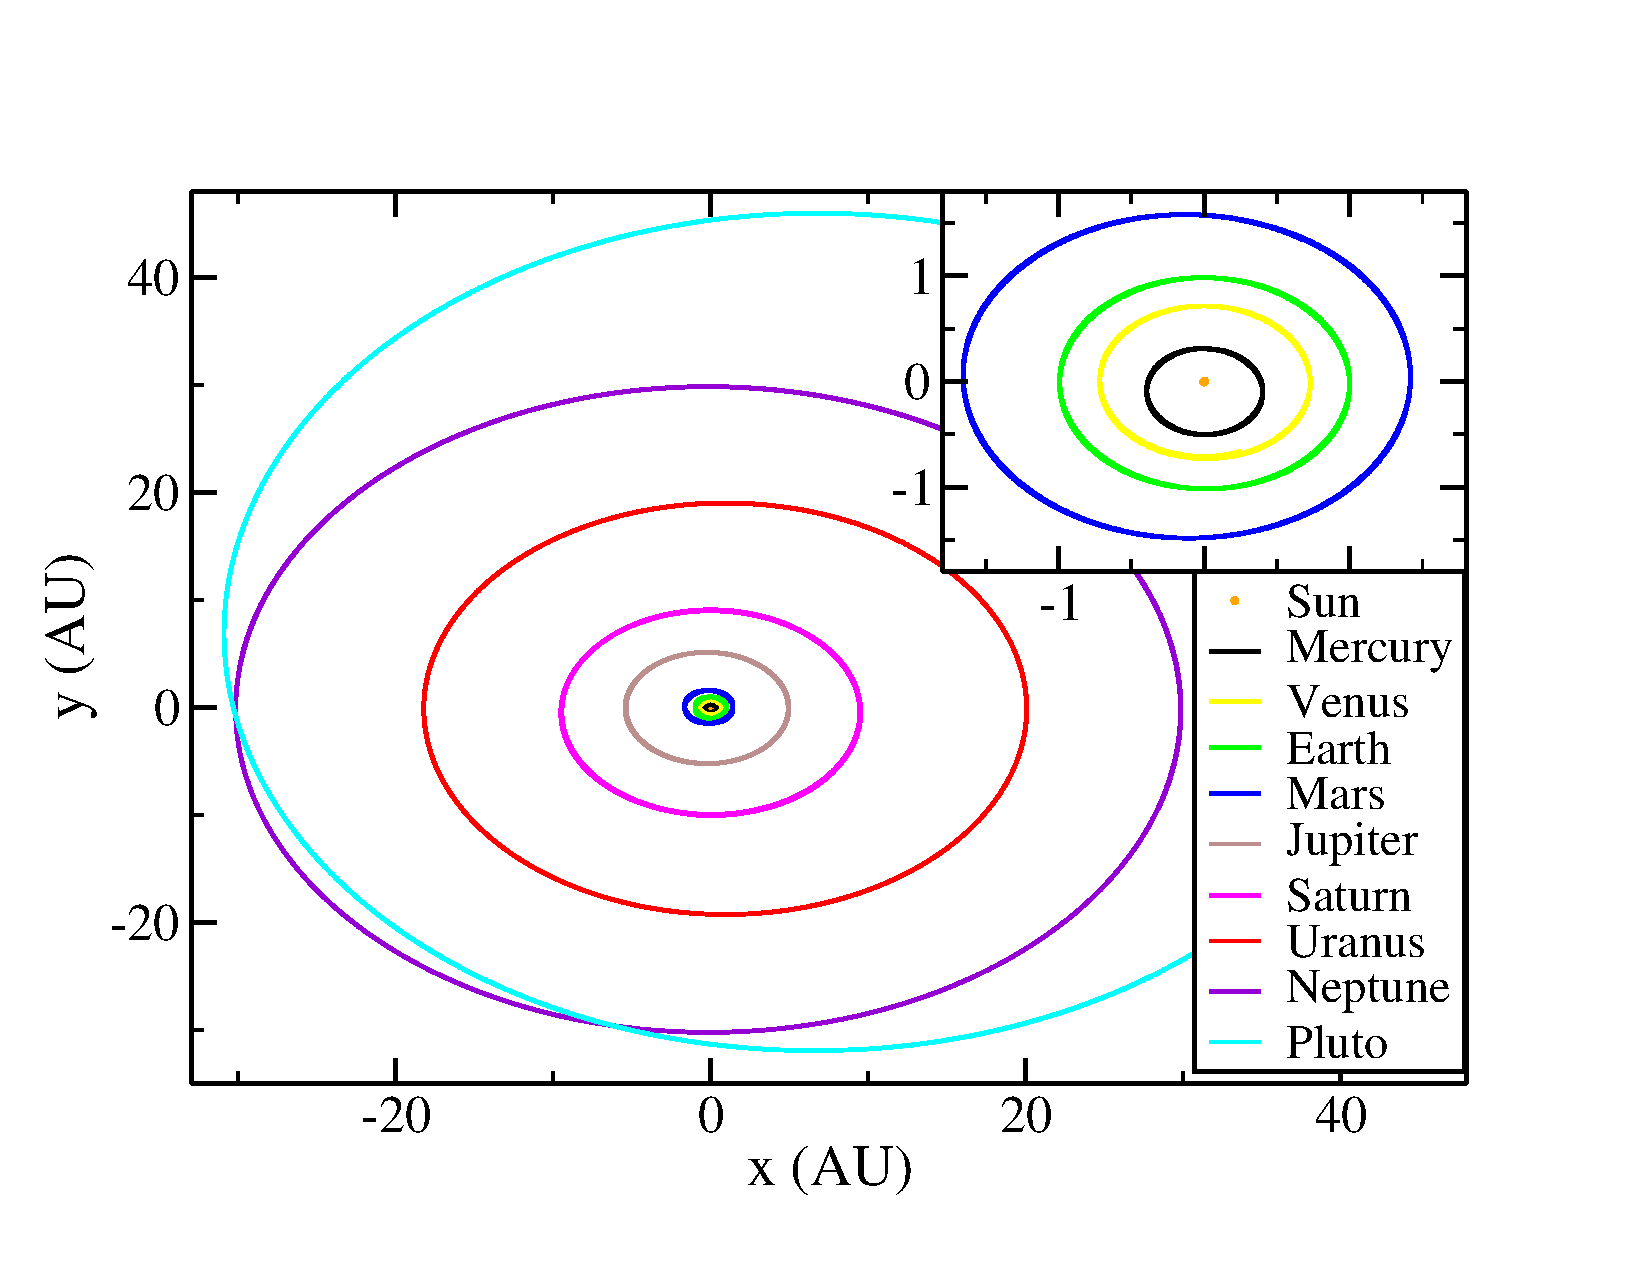
\includegraphics[scale=0.33]{all2.pdf}
\caption{Path of all planets in the solar system around the center of mass. The inset shows the paths of the smaller orbits.}
\label{all}
\end{figure}

\begin{table}[t]
\centering
\begin{tabular}{|c|c|c|}
\hline
Planet & ~Distance (AU) ~& ~Calculated Distance (AU) ~\\
\hline
Mercury&0.39 &0.385\\
Venus&0.72&0.716\\
Earth&1.00&1.010\\
Mars&1.52&1.525\\
Jupiter&5.20&5.189\\
Saturn&9.54&9.531 \\
Uranus&19.19&19.116\\
~Neptune~&30.06&30.030 \\
Pluto&39.53& 39.790\\
\hline
\end{tabular}
\caption{Comparison of expected and calculated distance from the sun.}
\label{comp}
\end{table}

\noindent numerically the paths of the planets in the solar system using Newton's law of gravitation. Two methods to calculate the differential equations were used, namely, the Euler method and the velocity Verlet method.

The Euler method was shown to be unstable in calculating the Earth's orbit in a system which only contained the Earth and sun. In contrast, the Verlet method was stable for practically all step sizes. While the Verlet method was slower, both methods took under one second, so the difference in timing was negligible. In addition, with the Verlet method we show the importance of the correct initial conditions, as too large of a velocity could cause the system to become unbound.

Next, we include Jupiter in the model, and explore the dependance of Earth's trajectory on the mass of Jupiter. The calculations are first performed with the physical mass of Jupiter and then with a mass 10 times larger and then 100 times. In all cases the final trajectories were indistinguishable, showing that the sun has the more substantial effect on the orbit of the planets.

There are a number of ways that our code can be improved upon, for example there are more algorithms that could have been explored, such as the Runge-Kutta method~\cite{RK}, which could prove to be more efficient. In addition, the precession of Mercury is known to be incorrect when only newtonian mechanics are considered, so an approximation of the effects of general relativity could be employed to correct for the differences. Finally, while the computation time for these examples were small, as moons and other various celestial bodies are added there may be a point in which parallelization of the Verlet algorithm as done in~\cite{omp} with OpenMP and MPI could be helpful. Although, it should be noted that this particular problem includes quite a bit of I/O manipulation, which would require additional effort.

Overall, we have demonstrated that using Newton's law of gravitation rather than general relativity yields fairly accurate results for the motion of the planets in our solar system. In addition, we have shown that the velocity Verlet algorithm is robust, especially for the chosen application. Finally, these results illustrate the importance of choosing the right tool for the job, as the Euler method failed to produce stable results for even the simplest of cases.



\bibliography{solar}
\end{document}

